\documentclass{article}
\usepackage{graphicx}
\usepackage[margin=1.5cm]{geometry}
\usepackage{amsmath}

\begin{document}

\title{Study Guide for Final: Elementary Statistics}
\author{Prof. Jordan C. Hanson}

\maketitle

\section{Formula Area}

\begin{enumerate}
\item Average/mean, definition 1: $\bar{x} = N^{-1} \sum_i x_i$
\item Median: the value below which are half of the frequencies.  Half of the frequencies are also above this value.
\item Mode: the value corresponding to the highest frequendy.
\item The quartiles $Q1$, $Q2$, and $Q3$ are the values that separate the frequencies into four bins of equal frequency. $Q2$ is equal to the median.  The IQR is $Q3 - Q1$.
\item The k-th percentile: the value below which k percent of the data is located.  Formula: $i = (k/100) (n+1)$, where $k$ is the percentile, $n$ is the total number of data, and $i$ is the integer location of the k-th percentile.
\item Finding the percentile of a data value: $(x+0.5*y)/n (100)$, where $x$ is the number of data values below the given data value, $y$ is the number of data values equal to the given one, and $n$ is the total number of data values.
\item Average/mean, definition 2: $\bar{x} = \sum_i^{M} f_{r,i} x_i$, where $x_i$ are the bin centers of a histogram, or the discrete random variable data values, and $f_{r,i}$ are the relative frequencies.  For a discrete random variable, $f_{r,i}$ is replaced with $p(x)$, the probability distribution function.
\item Probabilities of mutually exclusive and independent events: if two events have probabilities $p_1$ and $p_2$, then the probability that event 1 AND event 2 occur is $p_1 p_2$.  The probability that event 1 OR event 2 occurs is $p_1 + p_2$.
\item The standard deviation $s$ of a sample is 
\begin{equation}
s^2 = \frac{1}{N-1}\sum_{i=1}^{M} (x_i-\bar{x})^2
\end{equation}
\item The mean and standard deviation of the binomial distribution are $\mu = np$ and $\sigma = \sqrt{npq}$, respectively.
\item Let the PDF of the \textit{uniform distribution} be $p(x) = 1/(b+a)$.  The mean and standard deviation of this PDF are $\mu = (b+a)/2$ and $\sigma = \sqrt{(b-a)/12}$, respectively.
\item Let the PDF of the \textit{normal distribution} be $p(x) = \frac{1}{\sqrt{2\pi\sigma^2}} \exp(-0.5 (x-\mu)^2/\sigma^2)$.  The mean and standard deviation of this PDF are $\mu$ and $\sigma$, respectively.  We write $N(a,b)$ to refer to a normal distribution with mean $a$ and standard deviation $b$.
\item The z-score of a result drawn from $N(\mu,\sigma)$ is $z = (x_i - \mu)/\sigma$.  $P(|z| \leq 1) \approx 0.68)$, $P(|z| \leq 2) \approx 0.95)$, $P(|z| \leq 1) \approx 0.997)$.
\item \textbf{The central limit theorem} states that the means of samples of a population are distributed according to $N(\bar{x},\sigma_x/\sqrt{n})$, if the sample size is $n$.
\item \textbf{The confidence interval} [a,b] may be constructed such that a fraction CL of all confidence intervals with the same properties will contain the population mean, $\mu$.  The number CL is called the \textit{confidence level.}
\item Given the null hypothesis $H_0$ and an alternative hypothesis $H_a$, a \textbf{Type I error} is when we reject $H_0$ in favor of $H_a$, when $H_0$ is true.
\item Given the null hypothesis $H_0$ and an alternative hypothesis $H_a$, a \textbf{Type II error} is when we accept $H_0$ and reject $H_a$, when $H_0$ is false. 
\end{enumerate}

\clearpage

\begin{figure}[ht]
\centering
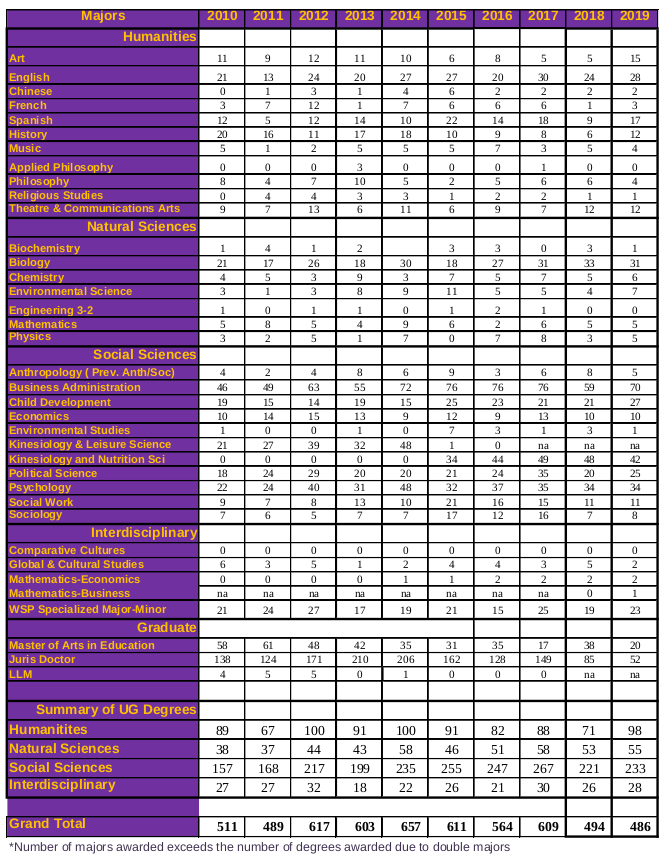
\includegraphics[width=0.8\textwidth]{figures/degree.png}
\caption{\label{fig:degree} Information regarding awarded Whittier College degrees.}
\end{figure}

\clearpage

\begin{enumerate}
\item Consider Fig. \ref{fig:degree}.  (a) Create a \textit{time-series} of the ratio of social science degrees to total degrees awarded versus time. (b) Create the same ratio, but for natural sciences. (c) Create a \textit{pareto chart} for the fraction of degrees in humanities, natural sciences, social sciences, and humanities awarded in 2019. (d) What mean number of physics degrees awarded per year, averaged over the past 10 years?  What is the standard deviation? \\ \vspace{4cm}
\item Consider Fig. \ref{fig:degree}.  (a) Create a histogram of the total degrees awarded each year, and determine the (b) quartiles of the data. \\ \vspace{3cm}
\item Suppose the number of biology degrees awarded at Whittier College awarded per year is described by $N(20,5)$.  (a) Suppose one year, we award 30 degrees in biology.  What is the z-score of this result?  (b) What is the probability of this result occuring by random chance? (c) What are the mean and standard deviation of the actual biology degrees across the last decade, according to Fig. \ref{fig:degree}? (d) What is the z-score of the most recent number of biology degrees? \\ \vspace{3cm}
\item Consider the following statistical claim: ``If we select a random Whittier College undergraduate student, the probability we will guess his or her major is 1/37, because there are 37 undergraduate majors.''  What is wrong with this claim, statistically? \\ \vspace{2cm}
\item Suppose we repeatedly measure the mean number of psychology degrees found in a randomly selected sample of size $n=100$ students.  (a) The mean is 10 and the standard deviation is 3.  What is the standard error in the mean, accordint to the CLT? (b) Construct a confidence interval that contains the true mean number of psychology degrees (per 100 students) that contains the true mean 95\% of the time.  \\ \vspace{2cm}
\item An office manager is interested in the mean number of emails each worker sends during his or her work day.  A survey of 30 employees is taken. The mean from the sample is 6.0 with a sample standard deviation of 4.0. (a) Construct the 95 percent confidence interval for the population mean, given the data.  (b) Graph the distribution of mean number of emails per day.  (c) Mark the confidence interval on the graph. \\ \vspace{2cm}
\item When a new drug is created, the pharmaceutical company must subject it to testing before receiving the necessary
permission from the Food and Drug Administration (FDA) to market the drug. Suppose the null hypothesis is “the drug is
unsafe.” What is the Type II Error?
\begin{itemize}
\item A: To conclude the drug is safe when in, fact, it is unsafe.
\item B: Not to conclude the drug is safe when, in fact, it is safe.
\item C: To conclude the drug is safe when, in fact, it is safe.
\item D: Not to conclude the drug is unsafe when, in fact, it is unsafe.
\end{itemize}
\item Suppose a new medicine moves ahead with human trials.  When people are given a placebo dose, 10 percent of them are ``cured.''  The fraction of patients cured with the new medicine is $20 \pm 5$ \%.  Suppose we construct a null hypothesis $H_0$: ``If the fraction of patients cured is greater than or equal to the result corresponding to two standard deviations above the placebo result, then the drug is effective.''  (a) Should we reject or confirm the null hypothesis?  At what significance level is this result? (b) Suppose there was a problem with the data, and the true rate of cure is actually $15 \pm 5$ \%.  What has happened to the significance level of the drug trial?
\end{enumerate}

\end{document}